%% ============================================================================
%%  SoftwareX Original Software Publication — pyvoa
%%  Based on the SoftwareX article template v4 (November 2023)
%%  Guide for authors: https://www.sciencedirect.com/journal/softwarex/publish/guide-for-authors
%%
%%  CONSTRAINTS TO RESPECT (SoftwareX, Guide for Authors):
%%    - Sections 1-5: max 6 pages / max 3000 words, counting abstract,
%%      running text, captions and footnotes; excluding title, authors,
%%      affiliations, references and metadata tables.
%%    - Max 6 figures. Abstract ca. 100 words. Max 6 keywords.
%%    - Code must be in a public *GitHub* repository (not GitLab).
%%  ============================================================================

\documentclass[preprint,12pt,a4paper]{elsarticle}

\usepackage[utf8]{inputenc}
\usepackage[T1]{fontenc}   % required: the funding sentence must keep its « » verbatim
\usepackage{amssymb}
\usepackage{graphicx}
\usepackage{listings}
\usepackage{xcolor}
\usepackage{booktabs}
\usepackage{etoolbox}
\usepackage[colorlinks=true,allcolors=blue]{hyperref}
\setlength{\parindent}{0pt}

%% ---------------------------------------------------------------------------
%%  DRAFT ANNOTATIONS
%%  All editorial notes are wrapped in \attn{...} / \attnpar{...}.
%%
%%  Two ways to turn them off, which must stay equivalent:
%%    - edit the line below to \togglefalse{draftmode}, or
%%    - leave it alone and build with
%%        latexmk -pdf -pretex='\def\paperfinal{1}' -usepretex main.tex
%%      which is what `make final` does. \providecommand cannot override a
%%      definition made by -pretex, so the command line wins and the source
%%      is provably the same for both PDFs.
%% ---------------------------------------------------------------------------
\providecommand{\paperfinal}{0}
\newtoggle{draftmode}
\ifdefstring{\paperfinal}{1}{\togglefalse{draftmode}}{\toggletrue{draftmode}}

\newcommand{\attn}[1]{%
  \iftoggle{draftmode}{\textcolor{red}{\textbf{[$\triangleright$ À TRAITER]} \textit{#1}}}{}%
}
\newcommand{\attnpar}[1]{%
  \iftoggle{draftmode}{\par\smallskip\noindent\fcolorbox{red}{red!5}{%
    \parbox{0.97\linewidth}{\textcolor{red}{\textbf{$\triangleright$ À TRAITER.} \textit{#1}}}}\par\smallskip}{}%
}

% Python code style
\lstdefinestyle{python}{
  language=Python,
  basicstyle=\ttfamily\small,
  keywordstyle=\color{blue},
  stringstyle=\color{red!70!black},
  commentstyle=\color{green!50!black},
  frame=single,
  framesep=4pt,
  backgroundcolor=\color{gray!5},
  breaklines=true,
  columns=fullflexible
}

\journal{SoftwareX}

\begin{document}
\renewcommand{\labelenumii}{\arabic{enumi}.\arabic{enumii}}

\attnpar{\textbf{État de conformité au 13 août 2026 --- à supprimer avant soumission.}
\emph{Dépôt.} Le commit \texttt{074f255} « docs: target SoftwareX instead of JOSS » a
levé l'ambiguïté de cible : \texttt{HANDOFF.md} déclare désormais SoftwareX (ISSN
2352-7110, type \emph{Original Software Publication}), \texttt{CITATION.cff} porte un
bloc \texttt{preferred-citation} SoftwareX prêt à décommenter, \texttt{AUTHORS} parle de
« software paper », et la seule mention JOSS résiduelle
(\texttt{CONTRIBUTING.md}~§8) ne concerne que la \emph{politique d'auteurat}, avec la
précision « whatever the venue » : c'est un usage légitime et neutre, à conserver. Le
dépôt est cohérent ; aucune action requise de ce côté.\\[3pt]
\emph{Article.} Structure conforme au canevas v4 : métadonnées, §1 Motivation and
significance, §2 Software description (2.1 architecture, 2.2 fonctionnalités,
2.3 historique et qualité), §3 Illustrative examples, §4 Impact, §5 Conclusions,
déclarations, remerciements, bibliographie. Corps $\approx$2\,400 mots sur 3\,000
autorisés ; 5 figures sur 6 ; 6 mots-clés sur 6 ; résumé 112 mots.
\textbf{Deux réserves} : (i)~le canevas officiel n'a pas pu être téléchargé
(sciencedirect renvoie 403 aux robots) --- \textbf{le récupérer et vérifier l'ordre et
l'intitulé exacts des rubriques}, notamment si des \emph{Highlights} sont demandés ;
(ii)~la section Impact demande des éléments que seuls les auteurs détiennent (voir §4).
Les cinq figures sont produites (2026-08-13) par
\texttt{examples/pyfiles/paper\_examples.py}, qui les écrit dans
\texttt{paper/figures/} ; \texttt{make figures} les régénère. En mise en page
Elsevier définitive (\texttt{final,5p,times,twocolumn}) l'article tient en
6~pages, tables de métadonnées et bibliographie comprises.\\[3pt]
\emph{Emplacement.} Ce fichier est destiné à \texttt{paper/main.tex} dans le dépôt, avec
\texttt{paper/Makefile} (\texttt{make draft} / \texttt{make final}),
\texttt{paper/README.md}, et \texttt{tests/test\_paper.py} qui vérifie à chaque
\emph{push} que l'article et le code disent la même chose : version C1/S1, nombre de
bases, plancher Python et dépendances de C7, bases et appels utilisés par les listings,
phrase de financement exigée par \texttt{AUTHORS}, titre de \texttt{CITATION.cff}, et
les limites SoftwareX (3\,000 mots, 6 figures, 6 mots-clés, références toutes citées).
Le test ne lit que des fichiers --- ni import de \texttt{geopandas}, ni réseau --- donc
il entre dans le \emph{job} hors-ligne existant sans nouvelle dépendance ni
modification de \texttt{ci.yml}, et se \emph{skip} de lui-même si \texttt{paper/} est
absent. Les deux PDF sortent de la même source : \texttt{make final} passe
\texttt{-pretex='\textbackslash def\textbackslash paperfinal\{1\}'}, rien n'est édité.
\textbf{Point à trancher} : ces annotations deviennent publiques. \texttt{HANDOFF.md}
fait déjà ce choix, mais l'appréciation portée en §4 sur la faiblesse des preuves
d'adoption est d'une autre nature. Alternative décrite dans \texttt{paper/README.md}.}

\textbf{Derniers commentaires lors du push git du papier par Claude} 
Still yours to decide, all recorded in HANDOFF.md: the Zenodo 0.5.0 metadata (§1), the issue-form check (§2), and inside main.tex the reproducible-capsule link for C3/S3, the Section 4 adoption evidence, the AI-use declaration, and a look at the official template's exact section list — plus the two I flagged but didn't act on, the openstreet default and contextily forcing matplotlib.

\begin{frontmatter}

\title{pyvoa: a Python framework for unified access, standardisation and
visualisation of open epidemiological data}

\attnpar{Titre. J'ai retiré « COVID-19 » et « pandemic » du titre : depuis la 0.5.0 le
catalogue contient mpox (\texttt{mpoxgh}), les infections respiratoires aiguës
(\texttt{sentinellesIRA}) et la surveillance des eaux usées (\texttt{sumeau}), et le nom
même du logiciel (Python \emph{Virus} Open Analysis) marque la sortie du cadre
strictement COVID en 2025. Le titre initial, centré COVID-19, sous-vend le logiciel et
contredit \texttt{CITATION.cff}. Variante plus courte possible :
« pyvoa: unified access to open epidemiological databases in Python ».\\[3pt]
\textbf{Point de cohérence dépôt/article.} Le bloc \texttt{preferred-citation} de
\texttt{CITATION.cff} (commenté, prêt pour SoftwareX depuis le commit \texttt{074f255})
porte un troisième titre : « pyvoa: a Python package for open analysis of viral
epidemiological data ». \textbf{Un seul titre doit survivre} : celui qui sera soumis. Le
répercuter dans \texttt{CITATION.cff} au moment de l'acceptation, en même temps que
volume, numéro d'article et DOI \texttt{10.1016/j.softx.\ldots}}

\author[upc,lpnhe]{Tristan~Beau}
\ead{tristan.beau@u-pariscite.fr}
\author[upc,msc]{Julien~Browaeys}
\ead{julien.browaeys@u-pariscite.fr}
\author[lpnhe]{Olivier~Dadoun\corref{cor1}}
\ead{olivier.dadoun@lpnhe.in2p3.fr}
\cortext[cor1]{Corresponding author.}

\address[upc]{Université Paris Cité, UFR de physique, F-75013 Paris, France}
\address[lpnhe]{LPNHE, CNRS/IN2P3, Sorbonne Université, Université Paris Cité,
UMR 7585, F-75005 Paris, France}
\address[msc]{MSC --- Matière et Systèmes Complexes, CNRS, Université Paris Cité,
UMR 7057, F-75013 Paris, France}

\attnpar{Auteurs et affiliations. Corrigées d'après \texttt{AUTHORS} et
\texttt{CITATION.cff} : chaque auteur porte bien deux affiliations pour T.~Beau et
J.~Browaeys, une seule pour O.~Dadoun. \textbf{(a)} Confirmer qui est
\emph{corresponding author} : le brouillon plaçait \texttt{\textbackslash corref} après
O.~Dadoun mais donnait l'adresse générique \texttt{contact@pyvoa.org} ; j'ai retenu
O.~Dadoun avec son adresse institutionnelle, ce qu'Elsevier préfère à une adresse de
projet. \textbf{(b)} Ajouter les ORCID à la soumission dans Editorial Manager
(0000-0002-2022-2140 ; 0000-0003-4405-9875 ; 0000-0002-2169-9725). \textbf{(c)} L'ordre
alphabétique retenu ici est celui d'\texttt{AUTHORS} ; si un ordre par contribution est
souhaité, il faut le décider maintenant et le répercuter dans \texttt{CITATION.cff},
\texttt{.zenodo.json} et \texttt{codemeta.json}.}

\begin{abstract}
pyvoa (Python Virus Open Analysis) is an open-source Python library giving
unified access to 24 open epidemiological databases --- among them Our World in
Data, Johns Hopkins University CSSE and Santé publique France --- through a
single five-keyword query grammar. Each source is described declaratively by a
JSON file and normalised into a common pandas or geopandas frame; a geolocation
layer reconciles country, region and sub-region names across sources and
supplies the geometries needed for mapping. Because the payloads are read from
the project's own Zenodo mirrors, series remain reproducible after their
original providers stop publishing. Time series, choropleth maps and histograms
are produced in two lines of code.
\end{abstract}

\attnpar{Résumé. 112 mots, contre $\sim$100 demandés par le \emph{template} v4 ; c'est
acceptable mais ne pas l'allonger. Il compte dans la limite globale de 3000 mots.
Vérifier le nombre de bases (24) au moment de la soumission : le décompte doit être
celui du tableau de \texttt{README.md}, seule source de vérité selon \texttt{HANDOFF.md}.}

\begin{keyword}
epidemiology \sep COVID-19 \sep open data \sep Python \sep data visualisation
\sep geolocation
\end{keyword}

\attn{Six mots-clés exactement, maximum autorisé ; « reproducible research » a été
retiré. Ils reprennent six des huit mots-clés de \texttt{CITATION.cff}.}

\end{frontmatter}


%% ============================================================================
%%  METADATA TABLES
%% ============================================================================

\section*{Metadata}
\label{metadata}

\begin{table}[!ht]
\small
\begin{tabular}{|l|p{5.6cm}|p{7.0cm}|}
\hline
\textbf{Nr.} & \textbf{Code metadata description} & \textbf{Metadata} \\
\hline
C1 & Current code version & v0.5.0 (released 2026-08-06) \\
\hline
C2 & Permanent link to code/repository used for this code version &
\url{https://github.com/pyvoa/pyvoa} \newline
archived release: \url{https://doi.org/10.5281/zenodo.21829902} \newline
concept DOI (all versions): \url{https://doi.org/10.5281/zenodo.21829901} \\
\hline
C3 & Permanent link to Reproducible Capsule &
\attn{à compléter --- voir note ci-dessous} \\
\hline
C4 & Legal Code License & MIT License \\
\hline
C5 & Code versioning system used & git \\
\hline
C6 & Software code languages, tools and services used &
Python~3; JSON database descriptors; pytest; ruff; GitHub Actions (lint, test
matrix on Python 3.10--3.13, weekly network tests); PyPI; Zenodo \\
\hline
C7 & Compilation requirements, operating environments \& dependencies &
Python~$\geq$~3.10. Required, with the lower bound each is tested against:
pandas~$\geq$~2.1.1, geopandas~$\geq$~1.0, shapely~$\geq$~2.0.2,
beautifulsoup4~$\geq$~4.11, numpy~$\geq$~1.26, pycountry~$\geq$~22.3.5,
pycountry\_convert~$\geq$~0.7.2, requests~$\geq$~2.28, unidecode~$\geq$~1.3,
lxml~$\geq$~4.9.3, IPython~$\geq$~8.10, contextily~$\geq$~1.3,
html5lib~$\geq$~1.1. Plotting backends (matplotlib, bokeh, seaborn) are optional and
detected at run time; \texttt{pip install pyvoa-full} installs them. Runs on
Linux, macOS and Windows, in a script, a console or a Jupyter notebook. \\
\hline
C8 & If available, link to developer documentation/manual &
\url{https://github.com/pyvoa/pyvoa/blob/main/CONTRIBUTING.md} \newline
\url{https://github.com/pyvoa/pyvoa/blob/main/README.md} \\
\hline
C9 & Support email for questions & contact@pyvoa.org \\
\hline
\end{tabular}
\caption{Code metadata.}
\label{codeMetadata}
\end{table}

\begin{table}[!h]
\small
\begin{tabular}{|l|p{5.6cm}|p{7.0cm}|}
\hline
\textbf{Nr.} & \textbf{(Executable) software metadata description} & \textbf{Metadata} \\
\hline
S1 & Current software version & v0.5.0 \\
\hline
S2 & Permanent link to executables of this version &
\url{https://pypi.org/project/pyvoa/0.5.0/} \newline
\url{https://pypi.org/project/pyvoa-full/} \\
\hline
S3 & Permanent link to Reproducible Capsule & \attn{idem C3} \\
\hline
S4 & Legal Software License & MIT License \\
\hline
S5 & Computing platforms/Operating Systems & Linux, macOS, Microsoft Windows;
any platform running Python~$\geq$~3.10, including hosted notebook services
(Google Colaboratory, Binder) \\
\hline
S6 & Installation requirements \& dependencies &
\texttt{pip install pyvoa} (library) or \texttt{pip install pyvoa-full}
(library and plotting backends) \\
\hline
S7 & If available, link to user manual &
\url{https://pyvoa.org} \newline
example notebooks: \url{https://github.com/pyvoa/pyvoa/tree/main/examples} \\
\hline
S8 & Support email for questions & contact@pyvoa.org \\
\hline
\end{tabular}
\caption{Software metadata.}
\label{executableMetadata}
\end{table}

\attnpar{Métadonnées. Le brouillon annonçait v0.4.2, Python~$\geq$~3.8, un wiki GitHub
(\texttt{/pyvoa/pyvoa/wiki}) qui n'existe pas, et une liste de dépendances incomplète :
tout cela est corrigé d'après \texttt{pyproject.toml} et \texttt{CHANGELOG.md}.
\textbf{Trois décisions restent à prendre.} \textbf{(1)~C3/S3, \emph{Reproducible
Capsule}} : le plus simple est de déposer sur Code Ocean une capsule exécutant le
notebook des exemples ; à défaut, donner le lien Binder
(\url{https://mybinder.org/v2/gh/pyvoa/pyvoa/main}), qui fonctionne déjà puisque
\texttt{requirements.txt} est maintenu à la racine pour cela, ou le lien Colab du
notebook \texttt{PyvoaForBeginners.ipynb}. Ne pas laisser la case vide : c'est un motif
de renvoi éditorial. \textbf{(2)} Si une version 0.5.1 est publiée avant soumission,
reprendre partout numéro, date et DOI de version --- le DOI \emph{concept}
\texttt{21829901} reste stable. \textbf{(3)} \texttt{HANDOFF.md} §1 signale que
l'enregistrement Zenodo 0.5.0 diverge encore de \texttt{CITATION.cff} (affiliations,
mots-clés, relation \texttt{continues}, wheel absente). À régler \emph{avant} de citer ce
DOI dans un article : un relecteur vérifiera la concordance, et c'est la seule
incohérence documentée qui subsiste entre le dépôt et ses métadonnées publiées.
\textbf{(4)} \texttt{HANDOFF.md} §2, mineur : confirmer, en étant connecté, que les
formulaires d'issue s'affichent bien sur GitHub, et sortir le numéro de version figé de
\texttt{bug\_report.yml}.}


%% ============================================================================
%%  1. MOTIVATION AND SIGNIFICANCE
%% ============================================================================

\section{Motivation and significance}
\label{sec:motivation}

The COVID-19 pandemic produced open epidemiological data at an unprecedented
scale. Global aggregators --- the Johns Hopkins University Center for Systems
Science and Engineering (JHU CSSE)~\cite{dong2020,dong2022} and Our World in
Data (OWID)~\cite{mathieu2021} --- and national agencies such as Santé publique
France, the Robert Koch Institut or the Italian Dipartimento della Protezione
Civile all published daily series. They did so, however, with incompatible file
formats, column vocabularies, temporal granularities and, above all,
incompatible geographic labels.

Two consequences follow, and pyvoa addresses both.

\textbf{Heterogeneity.} Comparing two sources means reconciling them by hand.
Country names differ (\texttt{United States} / \texttt{US} / \texttt{USA}),
sub-national units are keyed sometimes by name and sometimes by code, cumulative
and incident quantities are mixed, and equivalent indicators carry different
names. This reconciliation is repeated independently by every analyst, is rarely
published with the analysis, and is a frequent source of silent error. It also
puts the data out of reach of the audiences for whom these series are most
instructive --- secondary-school and university students, science journalists,
and researchers from outside epidemiology.

\textbf{Impermanence.} The problem has since changed nature. JHU CSSE stopped
collecting on 10 March 2023~\cite{dong2022}; several national portals have been
retired or restructured, and URLs that anchored thousands of analyses no longer
resolve. Retrospective and comparative work on the pandemic --- which is now
most of the work being done --- therefore rests on sources that are no longer
where they were, and that a reviewer often cannot re-fetch. Long-term
accessibility has become the binding constraint on reproducibility.

Several Python and R tools give programmatic access to pandemic data.
\texttt{covid}~\cite{covid_pypi} and COVID19Py~\cite{covid19py} are thin
wrappers around a single upstream feed, with no visualisation and no geographic
layer. The COVIDcast Epidata API~\cite{reinhart2021} of the Delphi group offers
a rich, well-documented set of signals with genuine normalisation, but is
centred on the United States. \texttt{covid19.analytics}~\cite{ponce2020} covers
JHU data with analysis and plotting facilities, within the R ecosystem. Generic
dashboard frameworks such as Dash~\cite{dash} render anything but reconcile
nothing. None of them mirrors its payloads, so all of them degrade as their
upstream sources disappear. Table~\ref{tab:comparison} summarises the
comparison.

\begin{table}[!h]
\centering
\small
\begin{tabular}{lccccc}
\toprule
\textbf{Tool} & \textbf{Lang.} & \textbf{Sources} & \textbf{Geo.} & \textbf{Viz.} & \textbf{Mirrored} \\
\midrule
\texttt{covid}~\cite{covid_pypi}            & Python & 2   & --         & --         & -- \\
COVID19Py~\cite{covid19py}                  & Python & 1   & --         & --         & -- \\
COVIDcast~\cite{reinhart2021}               & Py/R   & 10+ & US only    & \checkmark & -- \\
\texttt{covid19.analytics}~\cite{ponce2020} & R      & 2   & --         & \checkmark & -- \\
Dash~\cite{dash}                            & Python & --  & --         & \checkmark & -- \\
\textbf{pyvoa}                              & Python & 24  & \checkmark & \checkmark & Zenodo \\
\bottomrule
\end{tabular}
\caption{pyvoa and comparable tools. ``Sources'': databases exposed through one
interface; ``Geo.'': reconciliation of geographic identifiers across sources;
``Viz.'': built-in charts and maps; ``Mirrored'': payloads served from an
archive with a persistent identifier rather than from the upstream URL.}
\label{tab:comparison}
\end{table}

pyvoa answers both problems with one design. Twenty-four databases are
described declaratively, normalised into one schema, joined to a geolocation
layer that resolves names and supplies geometries, and served from the project's
own Zenodo deposits rather than from upstream URLs. A complete figure is two
lines of Python.

\attnpar{Références remplacées. Le brouillon citait \texttt{ritchie2020} (page web OWID)
et \texttt{covidcast} (site web Delphi) ; je les ai remplacés par les articles évalués
par les pairs correspondants (\emph{Sci. Data} pour OWID~\cite{mathieu2021},
\emph{PNAS} pour COVIDcast~\cite{reinhart2021}), plus citables dans un journal Elsevier.
Le brouillon citait aussi \texttt{heer2008} pour désigner Tableau : cet article porte sur
l'historique graphique en visualisation et n'est pas une référence de Tableau ; la
mention de Tableau a été supprimée, et un outil commercial propriétaire n'a de toute
façon pas sa place dans le tableau comparatif. Enfin ECDC et INSEE, cités dans
l'introduction du brouillon, ne correspondent à \emph{aucune} base du catalogue
(cf.~\texttt{pyvoa/data/}) : supprimés.}

\attnpar{À vérifier avant soumission. \textbf{(a)}~La date d'arrêt de JHU CSSE
(10~mars~2023) : contrôler dans~\cite{dong2022} ou sur le dépôt CSSEGISandData, et
harmoniser avec la formulation retenue. \textbf{(b)}~Le nombre de sources attribué à
COVIDcast (« 10+ ») dans le tableau~\ref{tab:comparison} : le vérifier sur la
documentation Delphi actuelle, ou remplacer par une formulation qualitative pour éviter
une contestation en relecture. \textbf{(c)}~Le tableau comparatif est le passage le plus
exposé d'un article SoftwareX : chaque « -- » doit être défendable. Vérifier en
particulier que \texttt{covid19.analytics} n'a effectivement pas de couche de
réconciliation géographique.}


%% ============================================================================
%%  2. SOFTWARE DESCRIPTION
%% ============================================================================

\section{Software description}
\label{sec:description}

\subsection{Software architecture}
\label{sec:architecture}

pyvoa is layered (Fig.~\ref{fig:architecture}). A user calls the front end; the
front end never touches a URL.

\textbf{Declarative source descriptions.} Every database is a JSON file in
\texttt{pyvoa/data/}. It carries the payload URL, the upstream reference URL,
the separator and decimal conventions, the columns to drop, the rows to select,
and a list of column descriptors mapping the source's own names onto pyvoa's
vocabulary --- with, for each, whether the series is cumulative and a
human-readable description. It also carries the geographic block: granularity
(\texttt{country}, \texttt{region}, \texttt{subregion}), the ISO~3166-1 alpha-3
code of the covered territory, and the location mode. \texttt{MetaInfo} and
\texttt{DataParser} interpret these files, so adding a source usually means
adding one JSON file and no Python at all.

\textbf{Geolocation.} Four classes handle geography. \texttt{GeoManager}
converts location names between the \texttt{iso2}, \texttt{iso3}, \texttt{name}
and \texttt{num} standards and absorbs the idiosyncratic spellings of individual
databases; all names pass through a normalisation that strips accents, collapses
separators and folds case, so \texttt{'esp'}, \texttt{'spain'} and
\texttt{'SPAIN'} resolve alike, as do \texttt{"cote d'ivoire"} and
\texttt{"Côte d'Ivoire"}. \texttt{GeoRegion} resolves supranational
groupings --- the UN M49 regions, plus the European Union, G7, G8, G20, G77,
OECD, BRICS, the Commonwealth and eight African and Latin American economic
communities --- so that a whole grouping is a single \texttt{where} argument.
\texttt{GeoCountry} provides sub-national units and their geometries for the
countries covered at that granularity, in main, dense or exploded variants so
that overseas territories can be drawn or set aside. \texttt{GPDBuilder} then
joins the epidemiological frame to the geometries and returns a geopandas
object. Formally, the layer implements
%
\begin{equation}
G:\ (\textit{source\_id},\ \textit{raw\_name}) \longrightarrow
(\textit{iso\_code},\ \textit{display\_name},\ \textit{geometry}),
\label{eq:geomapping}
\end{equation}
%
applied on loading, so that changing database leaves geographic identifiers
unchanged. The layer is importable on its own and useful outside epidemiology.

\textbf{Front end and visualisation.} \texttt{pyvoa.front} exposes a singleton's
methods at module level, so that the API reads as plain functions. Plotting
backends --- matplotlib~\cite{hunter2007}, bokeh~\cite{bokeh} and
seaborn~\cite{waskom2021} --- are optional imports probed at run time: the
library returns data with none of them installed, and reports a missing backend
rather than failing on import.

\begin{figure}[!h]
\centering
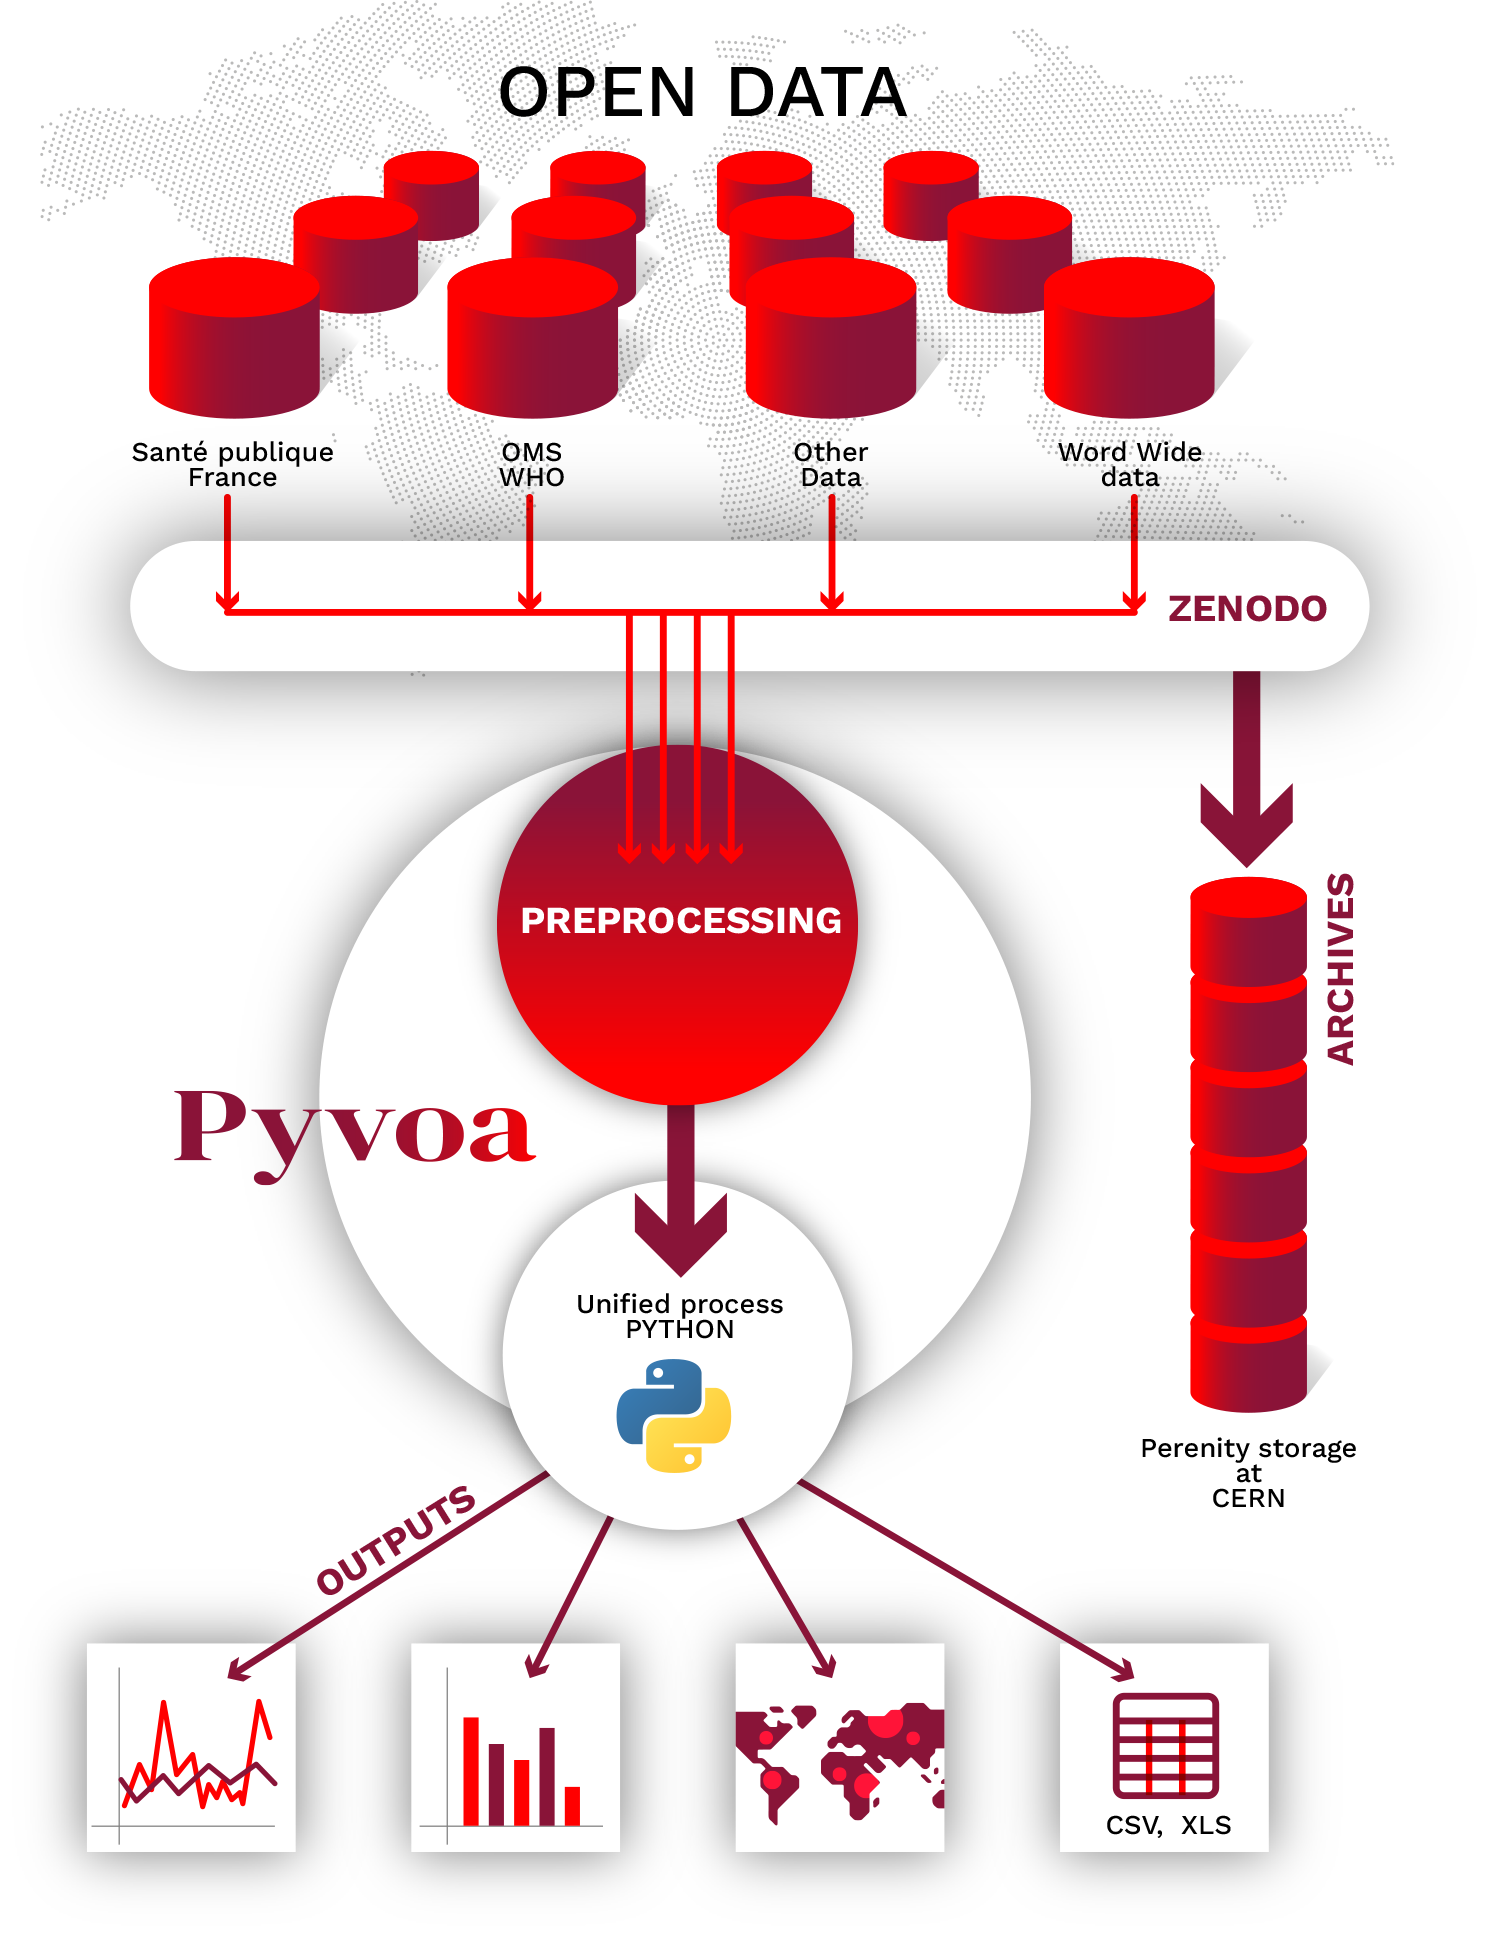
\includegraphics[width=0.5\textwidth]{figures/architecture.png}
\attn{figure matricielle (1500$\times$1934~px, RGBA). Elsevier demande 300~dpi
minimum pour un dessin au trait : à cette largeur elle passe, mais une version
vectorielle (PDF/EPS) serait préférable.}
\caption{Architecture of pyvoa. Upstream providers are mirrored on Zenodo; JSON
descriptors drive the parser; the geolocation layer reconciles names and adds
geometries; the front end exposes one query grammar and three chart families.}
\label{fig:architecture}
\end{figure}

\subsection{Software functionalities}
\label{sec:functionalities}

\textbf{One query grammar.} Four functions --- \texttt{get()},
\texttt{plot()}, \texttt{map()} and \texttt{hist()} --- take the same five
keywords, after \texttt{setwhom()} has selected a database and, for charts,
\texttt{setvis()} a backend:
\texttt{where} (one place, a list of places, or a grouping),
\texttt{which} (an indicator of the selected database),
\texttt{what} (\texttt{current}, \texttt{daily} or \texttt{weekly}),
\texttt{when} (a date or a \texttt{begin:end} range, \texttt{dd/mm/yyyy}), and
\texttt{option} (\texttt{sumall}, \texttt{nonneg}, \texttt{smooth7}, or
normalisation by population at six scales, combinable in a list).
\texttt{get()} additionally takes \texttt{output}, returning a pandas or
geopandas frame, a list, a dict or an array; \texttt{input} accepts an external
frame, so pyvoa charts data it did not fetch.

\textbf{Introspection.} Every vocabulary is enumerable at run time ---
\texttt{listwhom()}, \texttt{listwhich()}, \texttt{listwhere()},
\texttt{listwhat()}, \texttt{listoption()}, \texttt{listvis()},
\texttt{listoutput()} --- each returning a plain list, and \texttt{whattodo()}
returning the whole keyword-value matrix as a frame. Discovery needs no
documentation lookup, which matters for the teaching use described in
Section~\ref{sec:impact}.

\textbf{Charts.} \texttt{plot()} draws \texttt{date}, \texttt{compare},
\texttt{versus}, \texttt{spiral} and \texttt{yearly} views; \texttt{hist()}
draws histograms by location or by value, and pie charts; \texttt{map()} draws
choropleths over standard or dense geometries, with a date slider under bokeh.
Titles, legends, watermarks and \texttt{savefig()} behave identically across
backends, and \texttt{setbatch()} renders without opening a window.

\textbf{Caching and mirroring.} Downloads are cached under
\texttt{\textasciitilde/.cache/pyvoa.data\_<user>/} with CRC32 invalidation; a
file below 1000 characters is treated as a failed download and re-fetched.
Since v0.5.0 the payloads themselves are read from the project's Zenodo
deposits, the upstream URL being retained in the descriptor for provenance.
A series therefore stays fetchable, and an analysis re-runnable, after its
provider stops publishing.

\textbf{Errors.} \texttt{PyvoaError} is the library's single exception type; it
renders a coloured banner at construction, so the message reaches a notebook
user even when the traceback is hidden. Verbosity has three levels.

\attnpar{Points à confirmer dans cette section. \textbf{(a)}~L'article annonce que le
paquet \texttt{pyvoa} seul retourne des données sans backend graphique. C'est ce
qu'affirment \texttt{README.md} et \texttt{CLAUDE.md} ; le vérifier réellement dans un
environnement neuf (\texttt{pip install pyvoa} puis \texttt{get()}), car c'est une
affirmation vérifiable par un relecteur en trois minutes. \textbf{(b)}~\texttt{CLAUDE.md}
signale que \texttt{front.merger()} appelle une méthode inexistante. \emph{Traitement
différé, selon décision des auteurs} : l'article n'en fait donc aucune mention, ce qui
est la conduite correcte --- ne pas documenter une API non fonctionnelle. Noter
simplement que l'exposition subsiste, \texttt{merger} étant publique.
\textbf{(c)}~Le backend folium existe dans le code (\texttt{visu\_folium.py}) mais a été
retiré de la liste annoncée en 0.4.0 : ne pas le mentionner, ce qui est le cas ici ;
vérifier que la figure~1 ne le fait pas non plus. \textbf{(d)}~Confirmer que
\texttt{seaborn}, cité ici comme backend, est bien installé par \texttt{pyvoa-full}.
\textbf{(e)}~\emph{Réglé le 2026-08-13} : \texttt{pyproject.toml} porte désormais un
plancher testé sur chaque dépendance directe, vérifié par le \emph{job} CI
\texttt{minimum}. La table~C7 les reprend un à un ; les mettre à jour ensemble.
\textbf{(f)}~Sur le point (a) : \texttt{contextily}, dépendance \emph{requise},
exige lui-même \texttt{matplotlib}. Un \texttt{pip install pyvoa} installe donc
toujours matplotlib, et l'affirmation « la bibliothèque renvoie des données sans
aucun backend » décrit le comportement du code, pas ce qu'un utilisateur obtient.
Formulation plus sûre : les backends sont sondés à l'exécution et leur absence est
signalée au lieu de casser l'import.}

\subsection{Development history and quality assurance}
\label{sec:history}

pyvoa is the third name of one continuous project, developed throughout by the
same authors. \emph{CoCoA} (Covid Collaborative Analysis) began at the Data
Against COVID-19 hackathon of April 2020 with the aim it still has: unified
access to pandemic data for people who are not data specialists. It was renamed
\emph{PyCoA} (Python Covid Analysis) in November 2020 and developed under that
name until March 2025, accumulating some 1900 commits --- the multi-database
front end and the \texttt{GeoCountry} class in 2021, normalisation by
population, yearly and spiral plots in 2022, the JSON database descriptors in
2023, the matplotlib and seaborn backends in 2024. In early 2025 the
COVID-specific vocabulary was removed from the code base and the project became
\emph{pyvoa}, Python Virus Open Analysis: the point at which it stopped being
about one virus.

Version 0.5.0 (August 2026) is the first release prepared for external scrutiny.
The catalogue grew from 12 to 24 databases; payloads moved to the Zenodo
mirrors; packaging moved to PEP~621; an offline test suite was added, in which
any test needing an upstream server must be marked and is deselected by default,
so that a test cannot silently start depending on the network; and continuous
integration on GitHub Actions runs linting, the suite on Python 3.10 to 3.13,
and the network tests on a weekly schedule. Releases are published on PyPI and
archived on Zenodo with a concept DOI. The repository carries
\texttt{CITATION.cff}, \texttt{codemeta.json}, \texttt{.zenodo.json},
contribution and conduct guidelines, and a changelog covering every release
since 0.1.0 as well as the CoCoA and PyCoA years --- the only public record of a
history whose middle repository is private.

\attnpar{Section ajoutée (absente du brouillon). Elle répond directement à deux critères
de relecture SoftwareX --- maturité et pérennité du logiciel --- et vaut mieux que de
laisser croire que le projet date de 2025. \textbf{Deux vérifications} :
\textbf{(a)}~le brouillon initial affirmait un renommage « en 2023 », ce que reprend
aussi la page presse de pyvoa.org ; le \texttt{CHANGELOG.md} et \texttt{AUTHORS} datent
le renommage de février--mars~2025 (dernier commit pycoa : 2025-03-24). J'ai retenu 2025.
\textbf{Trancher, puis corriger pyvoa.org} pour éviter une incohérence entre l'article et
le site cité en métadonnée S7. \textbf{(b)}~Le chiffre de $\sim$1900 commits pour PyCoA
vient du \texttt{CHANGELOG.md} (1924 sur la ligne principale) ; comme le dépôt est privé,
ce nombre n'est pas vérifiable par un tiers. Soit on l'assume tel quel, soit on écrit
« some 1900 commits, recorded in the project's changelog ».}


%% ============================================================================
%%  3. ILLUSTRATIVE EXAMPLES
%% ============================================================================

\section{Illustrative examples}
\label{sec:examples}

The four examples below are drawn from the notebooks shipped with the package
and run in a plain Jupyter session after \texttt{pip install pyvoa-full}.

\subsection*{Example 1 --- comparing countries}

\begin{lstlisting}[style=python]
import pyvoa.front as pf
pf.setwhom('owid')            # Our World in Data, worldwide, by country
pf.setvis('matplotlib')
pf.plot(which='total_deaths', where='European Union',
        what='daily', option='smooth7')
\end{lstlisting}

\texttt{where='European Union'} expands to the member states through
\texttt{GeoRegion}; \texttt{what='daily'} differentiates the cumulative series
the source publishes; \texttt{option='smooth7'} applies a weekly rolling mean,
removing the reporting-day artefact visible in every national series
(Fig.~\ref{fig:timeseries}).

\begin{figure}[!h]
\centering
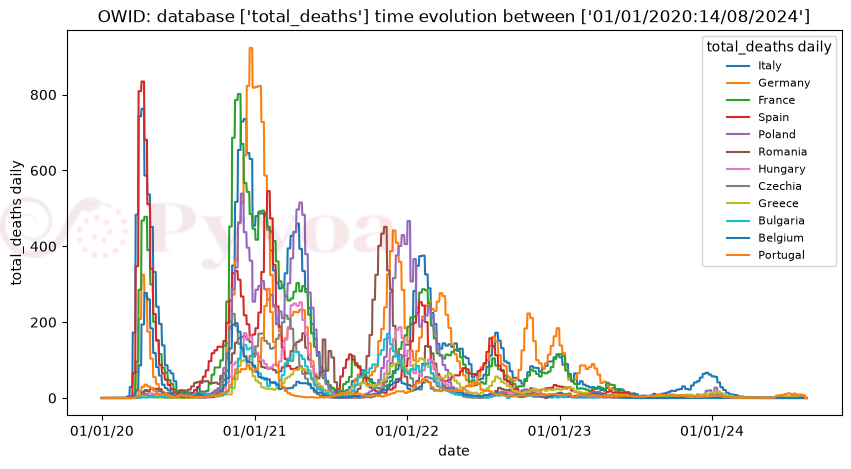
\includegraphics[width=0.9\textwidth]{figures/fig2_timeseries_eu.png}
\caption{Example 1. Daily COVID-19 deaths in the European Union member states,
seven-day smoothed, from Our World in Data.}
\label{fig:timeseries}
\end{figure}

\subsection*{Example 2 --- mapping a grouping}

\begin{lstlisting}[style=python]
pf.setwhom('jhu')             # Johns Hopkins CSSE, worldwide
pf.map(which='tot_confirmed', where='OECD',
       what='daily', when='01/12/2022', tile='positron')
\end{lstlisting}

One keyword selects the OECD member states, and the geolocation layer
supplies their geometries; the JHU series is read from its Zenodo mirror, the
upstream collection having ended in March 2023 (Fig.~\ref{fig:map}).

\begin{figure}[!h]
\centering
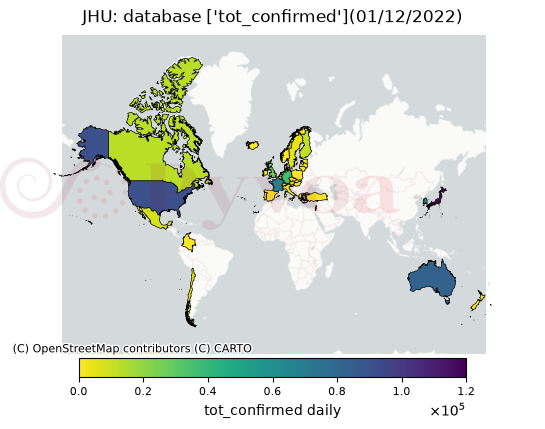
\includegraphics[width=0.9\textwidth]{figures/fig3_map_oecd.png}
\caption{Example 2. Daily confirmed COVID-19 cases across OECD member states on
1~December 2022, from the Johns Hopkins CSSE mirror.}
\label{fig:map}
\end{figure}

\subsection*{Example 3 --- ranking, and leaving the framework}

\begin{lstlisting}[style=python]
pf.setwhom('owid')
pf.hist(which='total_people_vaccinated_per_hundred',
        where='Asia', typeofhist='location')

df = pf.get(which='total_people_vaccinated_per_hundred',
            where='Asia', output='pandas')
\end{lstlisting}

\texttt{typeofhist='location'} draws one bar per country, ranked by magnitude
rather than by name
(Fig.~\ref{fig:hist}). The second call returns the same selection as a pandas
frame~\cite{mckinney2010}, with one row per date and place and standardised
geographic keys: pyvoa is a starting point for an analysis, not an enclosure.

\begin{figure}[!h]
\centering
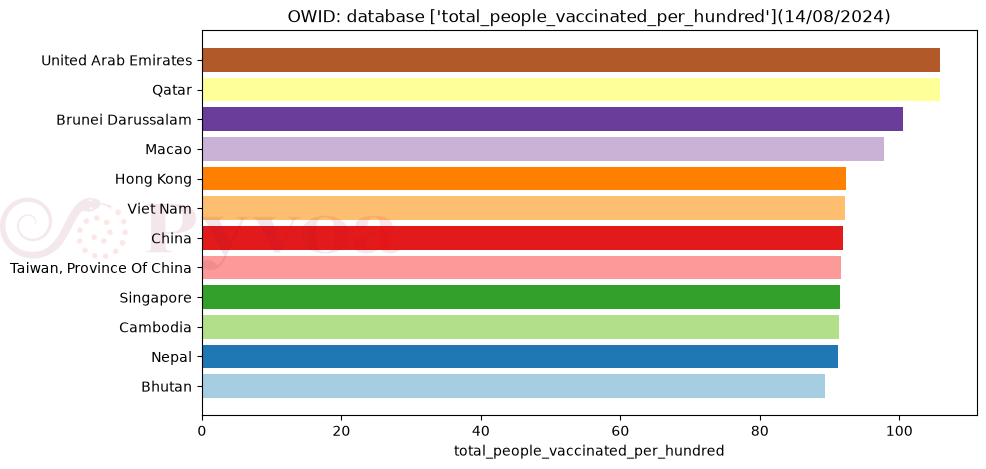
\includegraphics[width=0.85\textwidth]{figures/fig4_hist_asia.png}
\caption{Example 3. Share of the population having received at least one
COVID-19 vaccine dose, Asian countries, ranked.}
\label{fig:hist}
\end{figure}

\subsection*{Example 4 --- sub-national data, and beyond COVID-19}

\begin{lstlisting}[style=python]
pf.setwhom('spf')             # Sante publique France, departements
pf.map(which='cur_hosp', typeofmap='dense', tile='positron')

pf.setwhom('sumeau')          # SARS-CoV-2 in wastewater, France
pf.plot(which='ratio', typeofplot='yearly')
\end{lstlisting}

The same four keywords address a sub-national French source at
\emph{département} granularity, \texttt{typeofmap='dense'} bringing the overseas
\emph{départements} into the frame rather than dropping them
(Fig.~\ref{fig:mortality}), and then a wastewater surveillance series, whose
yearly overlay exposes the seasonal structure that a chronological axis hides.
Neither call required knowing anything about the two providers' file formats.

\begin{figure}[!h]
\centering
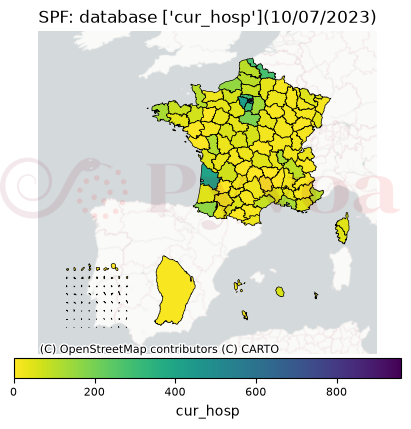
\includegraphics[width=0.49\textwidth]{figures/fig5a_map_spf_dense.png}\hfill
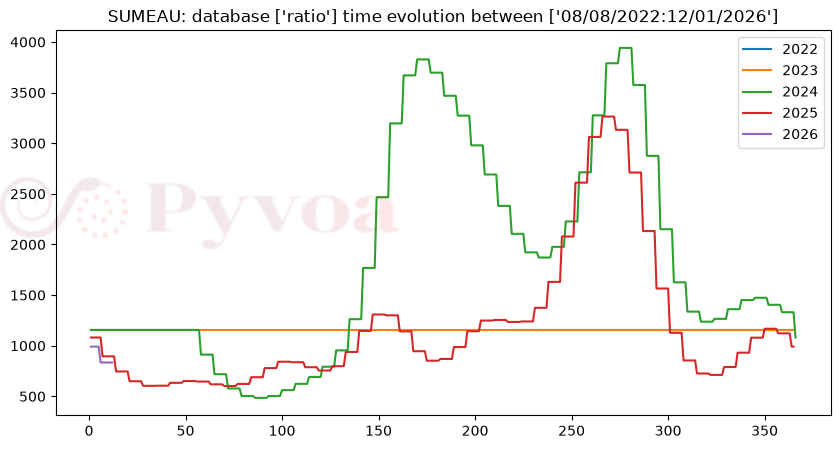
\includegraphics[width=0.49\textwidth]{figures/fig5b_sumeau_yearly.png}\\
\makebox[0.49\textwidth]{(a)}\hfill\makebox[0.49\textwidth]{(b)}
\caption{Example 4. (a) Patients hospitalised for COVID-19 by French
\emph{département}, dense geometry, from Santé publique France. (b) Yearly
overlay of the SARS-CoV-2 signal in French wastewater (SUM'EAU).}
\label{fig:mortality}
\end{figure}

\attnpar{Exemples entièrement réécrits --- le brouillon n'était pas exécutable.
\textbf{(1)}~L'exemple~4 portait sur une base \texttt{insee} qui \emph{n'existe pas} dans
\texttt{pyvoa/data/} (INSEE figurait dans PyCoA v2.20, mais pas dans le catalogue
pyvoa~0.5.0). Remplacé par \texttt{spf} + \texttt{sumeau}, ce qui illustre en outre la
sortie du cadre COVID. \textbf{(2)}~\texttt{typeofhist='byvalue'} a été renommé
\texttt{'value'} en 0.4.0 (cf.~\texttt{CHANGELOG.md}). Corrigé.
\textbf{(3)}~\texttt{total\_people\_fully\_vaccinated\_per\_hundred} n'existe pas dans
\texttt{owid.json} ; les colonnes disponibles sont
\texttt{total\_people\_fully\_vaccinated} et
\texttt{total\_people\_vaccinated\_per\_hundred}. Corrigé, et la légende de la
figure~\ref{fig:hist} ajustée en conséquence (« au moins une dose »).
\textbf{(4)}~\texttt{option=['smooth7','sumall']} du brouillon combinait un lissage et
une somme sur toutes les localisations, ce qui n'a pas de sens pour une superposition
annuelle par pays. Simplifié. \\[2pt]
\textbf{Il reste à exécuter les quatre exemples et à produire les figures.} Deux fichiers
sont fournis avec ce manuscrit : le notebook \texttt{PaperExamples.ipynb}, qui exécute
les quatre listings dans l'ordre de l'article et dont chaque cellule de code est
identique caractère pour caractère au listing imprimé --- de sorte qu'un relecteur peut
les comparer plutôt que les croire --- et le script \texttt{paper\_examples.py}, sa
version sans interface graphique (\texttt{matplotlib.use('Agg')}), doté d'un mode
\texttt{-{-}check} qui valide, sans rien tracer, que chaque base, indicateur, option et
regroupement cité existe dans la version installée. C'est exactement la classe d'erreur
qui rendait les listings du premier jet inexécutables. \textbf{Lancer
\texttt{python paper\_examples.py -{-}check} avant toute soumission}, et à nouveau après
toute montée de version. Vérifier en particulier :
que \texttt{when='01/12/2022'} tombe dans la couverture du miroir JHU ;
que \texttt{'OECD'} est bien accepté tel quel par \texttt{GeoRegion} (la casse est
normalisée, mais le confirmer) ; que \texttt{'Asia'} renvoie une liste non vide dans
\texttt{owid} ; et que \texttt{sumeau} accepte \texttt{typeofplot='yearly'} (base à
granularité \texttt{country}, une seule localisation : c'est la condition requise).
Générer les figures en PDF ou EPS vectoriel --- Elsevier refuse les captures d'écran
basse résolution. Déposer le notebook dans \texttt{examples/notebooks/} et le script dans
\texttt{examples/pyfiles/} du dépôt en ferait aussi la capsule reproductible demandée en
C3/S3, avec un lien Colab immédiat.\\[3pt]
\textbf{Défaut corrigé au passage} : le listing~3 supposait \texttt{owid} actif alors que
le listing~2 avait basculé sur \texttt{jhu}. L'appel \texttt{setwhom('owid')} a été
rétabli. C'est précisément le genre d'erreur qu'un relecteur exécutant le code trouve en
premier.}


%% ============================================================================
%%  4. IMPACT
%% ============================================================================

\section{Impact}
\label{sec:impact}

\textbf{Questions that become tractable.} Two kinds. First, cross-source
comparison. Because twenty-four databases share one schema and one geographic
key, a sub-national national source and an international country-level source
can be put side by side without writing a join: the French wastewater signal and
the reported incidence over the same territory, or a country's own agency series
against the aggregator's rendering of it --- a comparison that surfaces
reporting artefacts rather than assuming them away. Second, retrospective work
on sources that have ceased. The JHU series used in Section~\ref{sec:examples}
is no longer published; it is nonetheless fetched, by identifier, in one line.

\textbf{Existing questions pursued better.} The gain is on reproducibility
rather than on speed. An analysis written against pyvoa records which database,
which indicator, which pre-treatment and which options were used, in five
keywords that a reader can re-execute; and because the payload is read from an
archived copy carrying a persistent identifier~\cite{zenodo_pyvoa} rather than
from a live URL, re-execution years later returns the same numbers. This is what
a live endpoint cannot offer, and it is increasingly the limiting factor in
pandemic retrospectives.

\textbf{Daily practice, and who changes it.} The design constraint --- a
complete figure in two lines, every vocabulary enumerable at run time --- was
set for teaching, and the software has been used that way at Université Paris
Cité since 2020, in physics and data analysis courses. Students meet real,
heterogeneous, incomplete data on the first day rather than a cleaned teaching
set; \texttt{get()} then hands them a pandas frame, so the progression from
first figure to independent analysis happens without changing tool. The same
property serves science journalists and researchers from outside epidemiology,
the other audiences the project has targeted from the start.

\textbf{Uptake so far.} The project began at the Data Against COVID-19 hackathon
(April 2020) and was presented at Hackathon COVID --- Lutter Ensemble (April
2021) and at the 22nd Salon Culture et Jeux Mathématiques (May 2021). It was
covered by the CNRS MODCOV19 modelling platform~\cite{modcov19} and in
institutional communications of Sorbonne Université, Université Paris Cité and
LPNHE. \attn{compléter ici par les usages tiers documentés --- voir note}

\textbf{Reuse, and commercial status.} The geolocation layer is importable on
its own (\texttt{pyvoa.geo}) and contains nothing epidemiological: any dataset
keyed by country, region or French \emph{département} can be reconciled and
mapped with it. Extending the catalogue takes a JSON descriptor and no Python,
which is what makes a new disease a matter of hours rather than of a release
cycle. The software is distributed under the MIT licence, has no commercial
version and is not exploited commercially.

\attnpar{\textbf{Ce que le canevas SoftwareX attend exactement de la section 4.} Le
\emph{template} v4 demande d'y traiter, explicitement, les points suivants --- la
section ci-dessus est structurée dans cet ordre, un paragraphe par point :
\begin{enumerate}
\item les \emph{nouvelles} questions de recherche que le logiciel rend abordables ;
\item en quoi il améliore la poursuite de questions \emph{déjà} posées (précision,
      rapidité, reproductibilité, abaissement de la barrière d'entrée) ;
\item comment il modifie la pratique quotidienne de ses utilisateurs ;
\item les projets de recherche en cours qui l'utilisent, et son adoption effective ;
\item son éventuelle exploitation commerciale, ou l'absence de celle-ci.
\end{enumerate}
\textbf{Vérifier cette liste sur le canevas téléchargé} : \texttt{HANDOFF.md} §3 note que
sciencedirect.com renvoie 403 aux récupérations automatiques, la liste ci-dessus est donc
donnée de mémoire des versions v3/v4 et doit être recoupée avec le fichier réel obtenu
depuis \url{https://www.elsevier.com/journals/softwarex/23527110/guide-for-authors}. Le
canevas est \emph{obligatoire} : SoftwareX n'examine que les articles qui l'utilisent.}

\attnpar{\textbf{Impact --- c'est ici que se joue l'acceptation.} Un article SoftwareX est
évalué sur la démonstration d'usage, pas sur l'élégance du code, et le point~4 ci-dessus
est aujourd'hui le maillon faible : la liste hackathons/presse établit une visibilité,
pas une adoption. \textbf{Trois éléments à réunir, par ordre d'efficacité décroissante.}
\textbf{(a)}~\emph{Un usage tiers documenté} --- un travail publié, un mémoire, un cours
hors laboratoire, un article de presse ayant produit ses figures avec pyvoa ou PyCoA.
Une seule occurrence vérifiable pèse plus que toute la revue de presse. Chercher les
citations de PyCoA sur Google Scholar et HAL. \textbf{(b)}~\emph{Des chiffres
d'enseignement} : intitulés d'UE, niveaux (L2/L3/M1), effectifs annuels, années
concernées. « Utilisé en cours depuis 2020 » sans quantification sera lu comme une
autopromotion ; « environ N étudiants par an dans l'UE X » ne le sera pas.
\textbf{(c)}~\emph{Des chiffres d'adoption} : téléchargements PyPI (via
\url{https://pypistats.org/packages/pyvoa}), étoiles et forks GitHub, participants aux
Discussions. Attention : le dépôt affiche actuellement 0~étoile et 0~fork, et un
relecteur peut le constater --- ne citer ces métriques que si elles sont favorables, et
préférer alors PyPI. \textbf{(d)}~Le lien data.gouv.fr du brouillon initial renvoyait
vers une réutilisation \emph{PyCoa} : vérifier qu'il résout, et le citer en le
présentant comme tel, ou le retirer.}

\attnpar{\textbf{Suggestion de contenu pour le point~1.} L'exemple le plus convaincant
serait une figure ou une phrase montrant une question réellement traitée grâce à la
réconciliation multi-sources --- par exemple la comparaison
\texttt{sumeau} (eaux usées) / \texttt{spfnational} (incidence déclarée) sur la même
période, qui n'est faisable en deux lignes qu'avec pyvoa. Si vous disposez d'un tel
résultat, même modeste, il vaut mieux qu'un argument d'architecture. Le script
d'exemples fourni contient la requête correspondante.}


%% ============================================================================
%%  5. CONCLUSIONS
%% ============================================================================

\section{Conclusions}
\label{sec:conclusions}

pyvoa gives one Python interface to twenty-four open epidemiological databases.
Sources are described declaratively rather than coded, normalised into a common
frame, reconciled geographically by a layer that is useful in its own right, and
served from archived copies with persistent identifiers rather than from
upstream URLs that no longer resolve. A figure costs two lines; the underlying
frame is one call away, so the framework is a point of entry rather than a
boundary.

The pandemic's open data are now a historical record, and an increasingly
fragile one. Work ahead follows from that: widening the catalogue to further
respiratory and vector-borne diseases, deepening the sub-national geolocation
layer, and continuing to mirror sources before they disappear. Contributions ---
in particular new database descriptors --- are welcome through the
repository~\cite{pyvoa_github}, which documents the procedure.

\attn{Le brouillon annonçait aussi une API REST : rien dans le dépôt ne l'amorce, et une
feuille de route non engagée est un point faible en relecture. Retiré. Ne réintroduire
que si c'est décidé.}


%% ============================================================================
%%  DECLARATIONS
%% ============================================================================

\section*{CRediT authorship contribution statement}

\textbf{Tristan Beau:} Conceptualization, Methodology, Software, Project
administration, Writing -- original draft.
\textbf{Julien Browaeys:} Conceptualization, Software, Validation, Supervision,
Writing -- review \& editing.
\textbf{Olivier Dadoun:} Conceptualization, Software, Data curation,
Visualization, Writing -- review \& editing.

\attn{Rôles alignés sur le fichier \texttt{AUTHORS} du dépôt (taxonomie CRediT,
ANSI/NISO~Z39.104-2022), auxquels j'ai ajouté les rôles de rédaction, absents
d'\texttt{AUTHORS} puisqu'il décrit le logiciel et non l'article. À répartir réellement.}

\section*{Declaration of competing interest}

The authors declare that they have no known competing financial interests or
personal relationships that could have appeared to influence the work reported
in this paper.

\section*{Declaration of generative AI and AI-assisted technologies in the writing process}

\attnpar{Déclaration obligatoire, à compléter par les auteurs. Elsevier impose une
formulation en fin de manuscrit, avant les remerciements, uniquement pour l'usage d'IA
générative \emph{dans la rédaction}. Formulation type :\\[3pt]
\textit{« During the preparation of this work the authors used [outil] in order to
[tâche]. After using this tool, the authors reviewed and edited the content as needed
and take full responsibility for the content of the publication. »}\\[3pt]
Deux précisions utiles ici. \textbf{(1)}~L'usage d'assistants dans le \emph{code} ne
relève pas de cette déclaration (elle vise la rédaction), mais le dépôt en porte la
trace publique --- \texttt{CLAUDE.md}, \texttt{HANDOFF.md}, et le \texttt{CHANGELOG}
de la 0.3.1 qui indique que les docstrings ont été écrites avec assistance LLM. Un
relecteur les verra. Le plus sûr est de le mentionner brièvement et sans détour, ce qui
est aussi cohérent avec la politique éditoriale. \textbf{(2)}~Vérifier la formulation en
vigueur sur \url{https://www.elsevier.com/about/policies/publishing-ethics} au moment de
la soumission : elle a déjà été révisée deux fois.}

\section*{Acknowledgements}
\label{sec:acknowledgements}

This work was supported by the IdEx « Université Paris Cité 2022 »
(ANR-18-IDEX-0001) and by the « Institut Covid-19 Ad Memoriam » of Université
Paris Cité. The project originated at the Data Against COVID-19 hackathon
(April 2020). The authors thank the CNRS MODCOV19 platform, and CNRS/IN2P3,
Université Paris Cité and Sorbonne Université for institutional support.

\attnpar{\textbf{Ne pas modifier la première phrase.} Le fichier \texttt{AUTHORS} du
dépôt précise que cette formulation est une condition du financement et doit être reprise
telle quelle dans toute publication. Elle figure aussi dans \texttt{.zenodo.json}. Le
brouillon l'avait omise : c'était le manquement le plus sérieux du texte initial.
Renseigner par ailleurs les financeurs dans le formulaire Editorial Manager (Funder
Registry : Agence Nationale de la Recherche, ANR-18-IDEX-0001).}


%% ============================================================================
%%  REFERENCES
%% ============================================================================

\begin{thebibliography}{00}

\bibitem{dong2020}
E.~Dong, H.~Du, L.~Gardner, An interactive web-based dashboard to track COVID-19
in real time, Lancet Infect.\ Dis.\ 20~(5) (2020) 533--534.
\url{https://doi.org/10.1016/S1473-3099(20)30120-1}.

\bibitem{dong2022}
E.~Dong, J.~Ratcliff, T.D.~Goyea, et~al., The Johns Hopkins University Center
for Systems Science and Engineering COVID-19 Dashboard: data collection process,
challenges and future enhancements, Can.\ J.\ Stat.\ 50~(4) (2022) 1418--1438.
\url{https://doi.org/10.1002/cjs.11744}.

\bibitem{mathieu2021}
E.~Mathieu, H.~Ritchie, E.~Ortiz-Ospina, et~al., A global database of COVID-19
vaccinations, Nat.\ Hum.\ Behav.\ 5 (2021) 947--953.
\url{https://doi.org/10.1038/s41562-021-01122-8}.

\bibitem{covid_pypi}
covid --- Python package to get information regarding the novel coronavirus,
\url{https://pypi.org/project/covid/}.

\bibitem{covid19py}
COVID19Py --- a tiny Python package for easy access to up-to-date coronavirus
data, \url{https://pypi.org/project/COVID19Py/}.

\bibitem{reinhart2021}
A.~Reinhart, L.~Brooks, M.~Jahja, et~al., An open repository of real-time
COVID-19 indicators, Proc.\ Natl.\ Acad.\ Sci.\ USA 118~(51) (2021) e2111452118.
\url{https://doi.org/10.1073/pnas.2111452118}.

\bibitem{ponce2020}
M.~Ponce, A.~Sandhel, covid19.analytics: An R package to obtain, analyze and
visualize data from the 2019 coronavirus disease pandemic, J.\ Open Source
Softw.\ 6~(60) (2021) 2995. \url{https://doi.org/10.21105/joss.02995}.

\bibitem{dash}
Plotly, Dash: a Python framework for building analytical web applications,
\url{https://dash.plotly.com/}.

\bibitem{mckinney2010}
W.~McKinney, Data structures for statistical computing in Python, in: Proc.\
9th Python in Science Conf., 2010, pp.~56--61.
\url{https://doi.org/10.25080/Majora-92bf1922-00a}.

\bibitem{hunter2007}
J.D.~Hunter, Matplotlib: a 2D graphics environment, Comput.\ Sci.\ Eng.\ 9~(3)
(2007) 90--95. \url{https://doi.org/10.1109/MCSE.2007.55}.

\bibitem{bokeh}
Bokeh Development Team, Bokeh: Python library for interactive visualization,
\url{https://bokeh.org/}.

\bibitem{waskom2021}
M.L.~Waskom, seaborn: statistical data visualization, J.\ Open Source Softw.\
6~(60) (2021) 3021. \url{https://doi.org/10.21105/joss.03021}.

\bibitem{modcov19}
T.~Beau, J.~Browaeys, O.~Dadoun, PyCoa: Python Covid Analysis, MODCOV19
(CNRS), 2022.
\url{https://modcov19.math.cnrs.fr/prepublications/2022_03_11_beau/}.

\bibitem{zenodo_pyvoa}
pyvoa community on Zenodo, \url{https://zenodo.org/communities/pyvoa}.

\bibitem{pyvoa_github}
T.~Beau, J.~Browaeys, O.~Dadoun, pyvoa: Python Virus Open Analysis, v0.5.0,
Zenodo, 2026. \url{https://doi.org/10.5281/zenodo.21829901}.
Repository: \url{https://github.com/pyvoa/pyvoa}.

\end{thebibliography}

\attnpar{Bibliographie. \textbf{(a)}~Passée de 20 à 15 entrées : les références non
citées dans le texte ont été supprimées (SoftwareX les refuse), ainsi que
\texttt{spf2020}, \texttt{insee2020}, \texttt{kluyver2016}, \texttt{geopandas},
\texttt{datagouv}, \texttt{lauer2023} et \texttt{heer2008}, devenues sans objet.
\textbf{(b)}~\texttt{ponce2020} : la référence du brouillon (JOSS 5(51):2363, 2020)
correspond à un autre article ; celle donnée ici (6(60):2995, 2021) est
\texttt{covid19.analytics}. \textbf{À revérifier} sur \url{https://joss.theoj.org}.
\textbf{(c)}~\texttt{covid\_pypi} et \texttt{covid19py} n'ont ni auteur fiable ni DOI ;
les noms d'auteurs du brouillon étaient invérifiables et ont été retirés. Envisager de
les citer en note de bas de page plutôt qu'en bibliographie. \textbf{(d)}~Elsevier
souhaite un DOI pour chaque référence qui en possède un : les six premières en ont, les
autres sont des logiciels ou des pages web, ce qui est admis. \textbf{(e)}~Passer en
BibTeX (\texttt{elsarticle-num}) plutôt qu'en \texttt{thebibliography} manuel avant
soumission, pour limiter les erreurs de saisie.}

\end{document}
